%!TEX root = ../thesis.tex
\subsection{Results}

We gathered nine different tutorials and recorded working through each tutorial in Photoshop. We then used MixT to automatically generate mixed media tutorials from these demonstrations. This section describes this corpus. The following section then evaluates the generated tutorials quantitatively and qualitatively.

Our tutorials came from both online and book sources: two from ``Adobe Photoshop CS5 Classroom in a Book,'' five from photoshopstar.com, one from makeuseof.com, and one from icanbecreative.com. All are popular resources for Photoshop learners. Two of the tutorials were also used in the formative user study. The selected tutorials had a total of 165 steps and covered all five command types: they contained 15 brushing/drawing operations, 14 control point manipulations, 30 parameter adjustments, 67 UI navigations, and 39 layer operations. The demonstrations were recorded on three different laptops running Photoshop in full screen with native resolutions of 1680x1050, 1440x900, and 1280x800 pixels.

Overall, the MixT tutorials that we generated exhibit the desired characteristics that we identified in our formative study: scannable steps, small but legible videos, visualized mouse operations, and user control over presentation format. We highlight some interesting results generated by MixT and also refer readers to the provided video figure, which has additional examples.

Scannability: The step-by-step layout of our tutorials makes them easy to scan. For example, at a glance, we see that the tutorial ``Turning an Image into an Old Photo'' involves several adjustment layer operations, while the tutorial ``Creating Artistic Effects'' involves more parameter adjustments and brushing commands.

Mouse visualization: Our mouse visualizations help clarify several interactions. They clearly communicate the difference between clicking and dragging, a distinction that is fundamental to operations such as path manipulation but hard to glean from screen capture video. For example, Figure~\ref{fig:mixt_results}A shows the difference between moving around the contour of an object without drawing a path (left), and dragging a Bézier handle to adjust a path segment (right). Mouse trails and click markers were also useful for showing the trajectory of lasso selections (Figure~\ref{fig:mixt_results}B).

Zoom and crop modes: For many steps, the zoom and crop videos offer clear legibility benefits over the normal video mode. In our corpus, zoom mode was especially valuable for highlighting actions on small buttons that occurred near the frame boundaries, e.g., in the layers palette (Figure~\ref{fig:mixt_results}C right). Such operations are easy to miss in a normal, scaled video (Figure~\ref{fig:mixt_results}C left). Crop mode was useful in showing the effect that parameter selection has on the canvas. Figure~\ref{fig:mixt_results}D shows two successive frames that illustrate how changing a layer's blending mode affects the image. Enlarging the canvas in these modes also helps users see the details of effects, such as applying the eraser tool on the canvas to enhance the underlying layer (Figure~\ref{fig:mixt_mouse}).

\begin{figure*}[t]
  \centering
  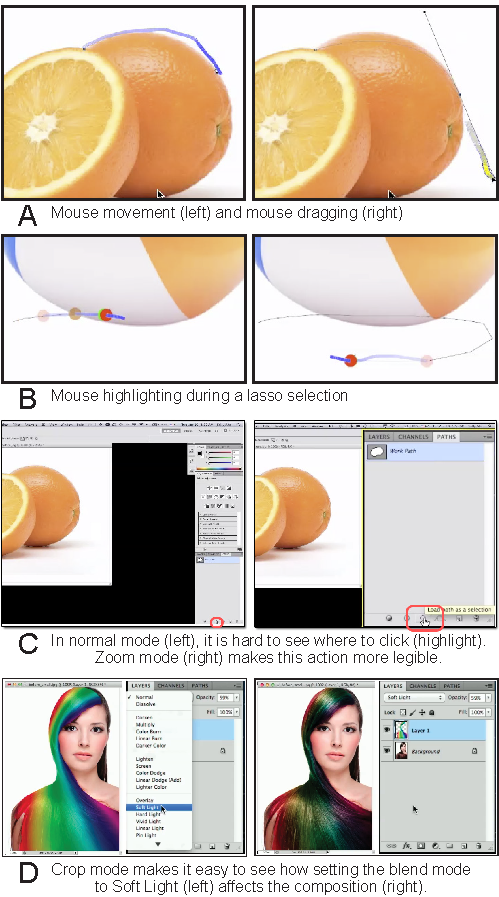
\includegraphics[width=0.67\textwidth]{\mixt/fig/mixt_results/mixt_results}
  \caption{Automatically-generated MixT results.}
  \label{fig:mixt_results}
\end{figure*}

